\chapter{Benchmarking}
\label{sec:benchmarking}

\section{Goal}
\section{Experimental Setup}

\begin{landscape}
\begin{table}[p!]
\begin{adjustbox}{width=19cm}
\rowcolors{2}{gray!13}{white}
\begin{tabular}{l|ll|p{46mm}p{67mm}}
\rowcolor{gray!26}
Name & Connector & Data Type & Goal & Description \\

\hline
seq-fifo & fifo1 & Integer & Tease out Proto overhead & alternate between putting and getting on single thread. measure RTT. Repeat for different sizes of data. Compare overhead to std::spsc channel \\

SIMO clone & N-replicator & BigClonable & check if getters are effectively cloning in parallel & repeatedly clone from a single putter in parallel \\

SIMO copy & N-replicator & BigCopyable & check if copying saves a lot of time vs cloning & repeatedly copy from a single putter in parallel \\

MO clone & N-keeper & BigClonable & Check if waiting for putter adds significant time & repeatedly clone from a memcell \\

counting & binary counter & BigClonable & Check how effective the refcounting is & binary counter circuit, moving memory between cells a hell of a lot. not much firing \\

MO fine & N-keeper fine & BigClonable & Check if coordinator is the bottleneck & have one rule per getter. each readiness causing a firing. \\

bitsets & N-keeper fine & BigClonable & fire every time, but after N-1 false guard evals by bitsets & N-keeper where only the last port and rule are active. effectively have to traverse all these dead rules each time \\

hashsets & N-keeper fine & BigClonable & check if the bitsets themselves helped & repeat bitset experiments, but modify Reo-rs to use stdlib hashsets instead \\

transform & transformer & int, float & overhead of createfromcall & \\

filter & filter & int & & \\

router & router & int & & \\

parallel & parallel & BitCopyable & concoct a scenario where data is moving in parallel as much as possible. & 

\end{tabular}
\end{adjustbox}
\caption[TODO]{TODO}	
\end{table}
\end{landscape}

\section{Results}

\subsection{Port Operation Overhead}

\begin{figure}
	\centering
	\makebox[\textwidth][c]{
		\begin{subfigure}[b]{0.63\textwidth}
			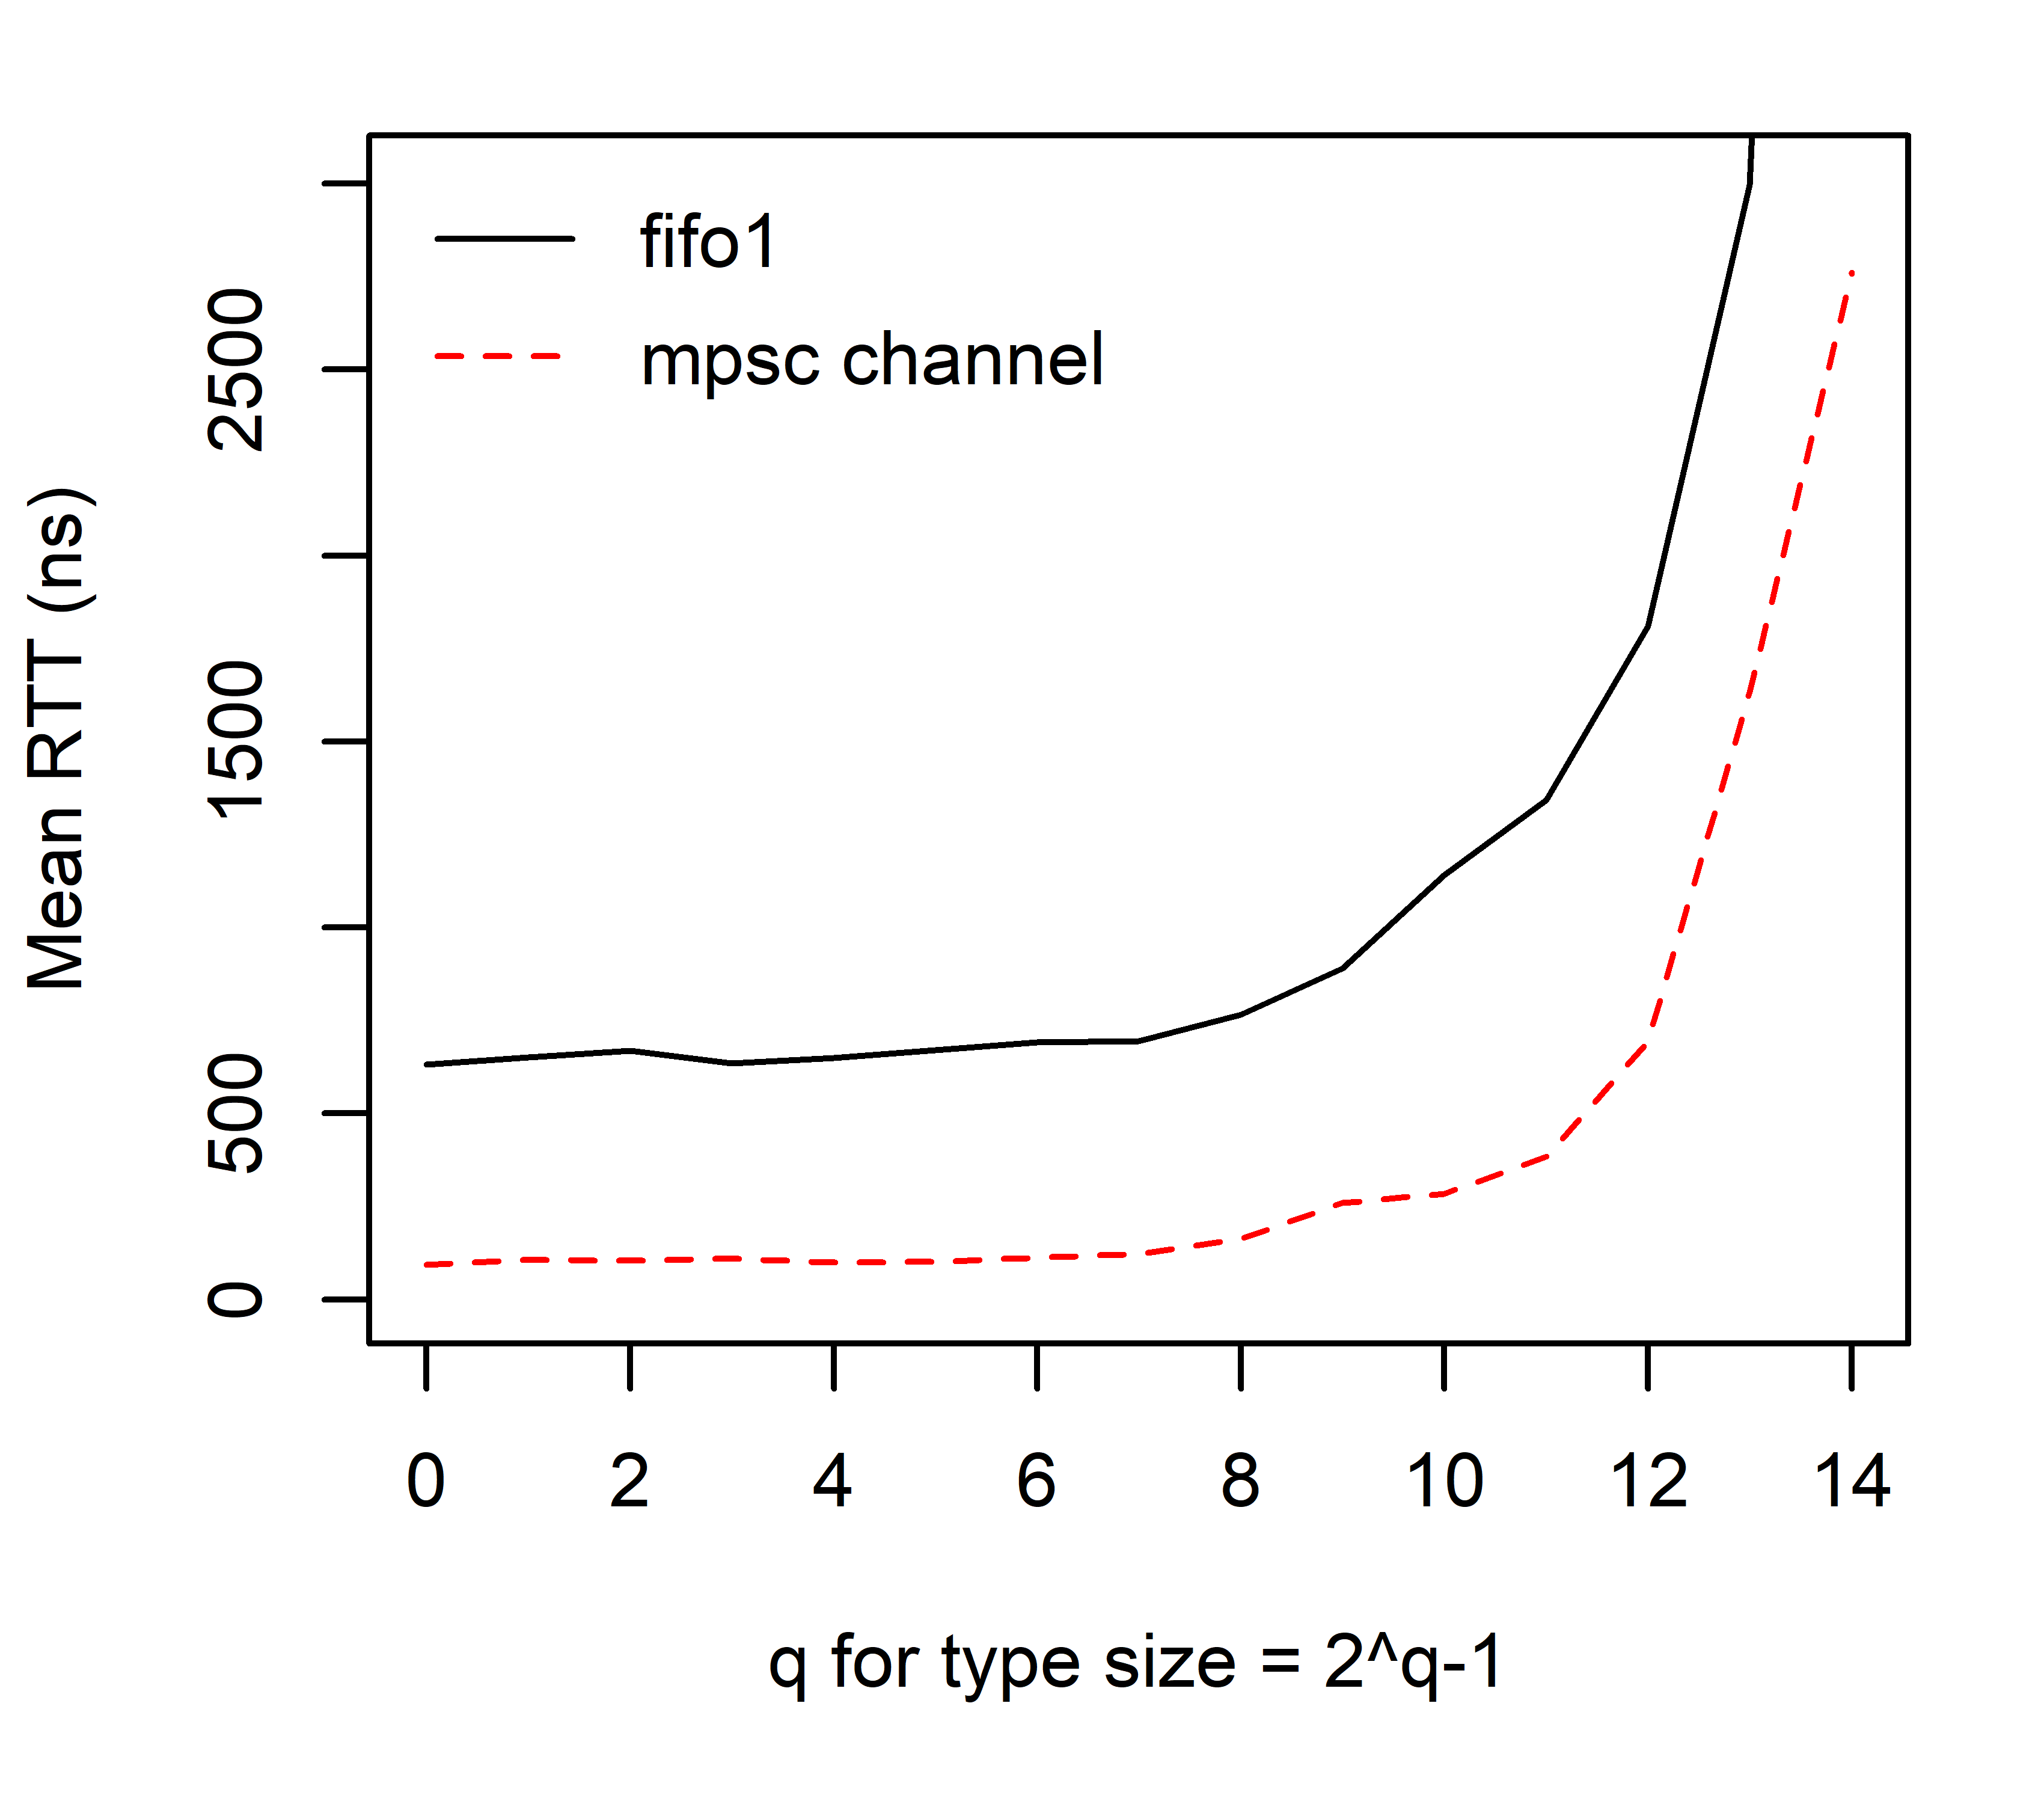
\includegraphics[width=\textwidth]{experiments/rtt_0.png}
			\caption{}
			\label{fig:exper_rtt_0}
		\end{subfigure}%
		\begin{subfigure}[b]{0.63\textwidth}
			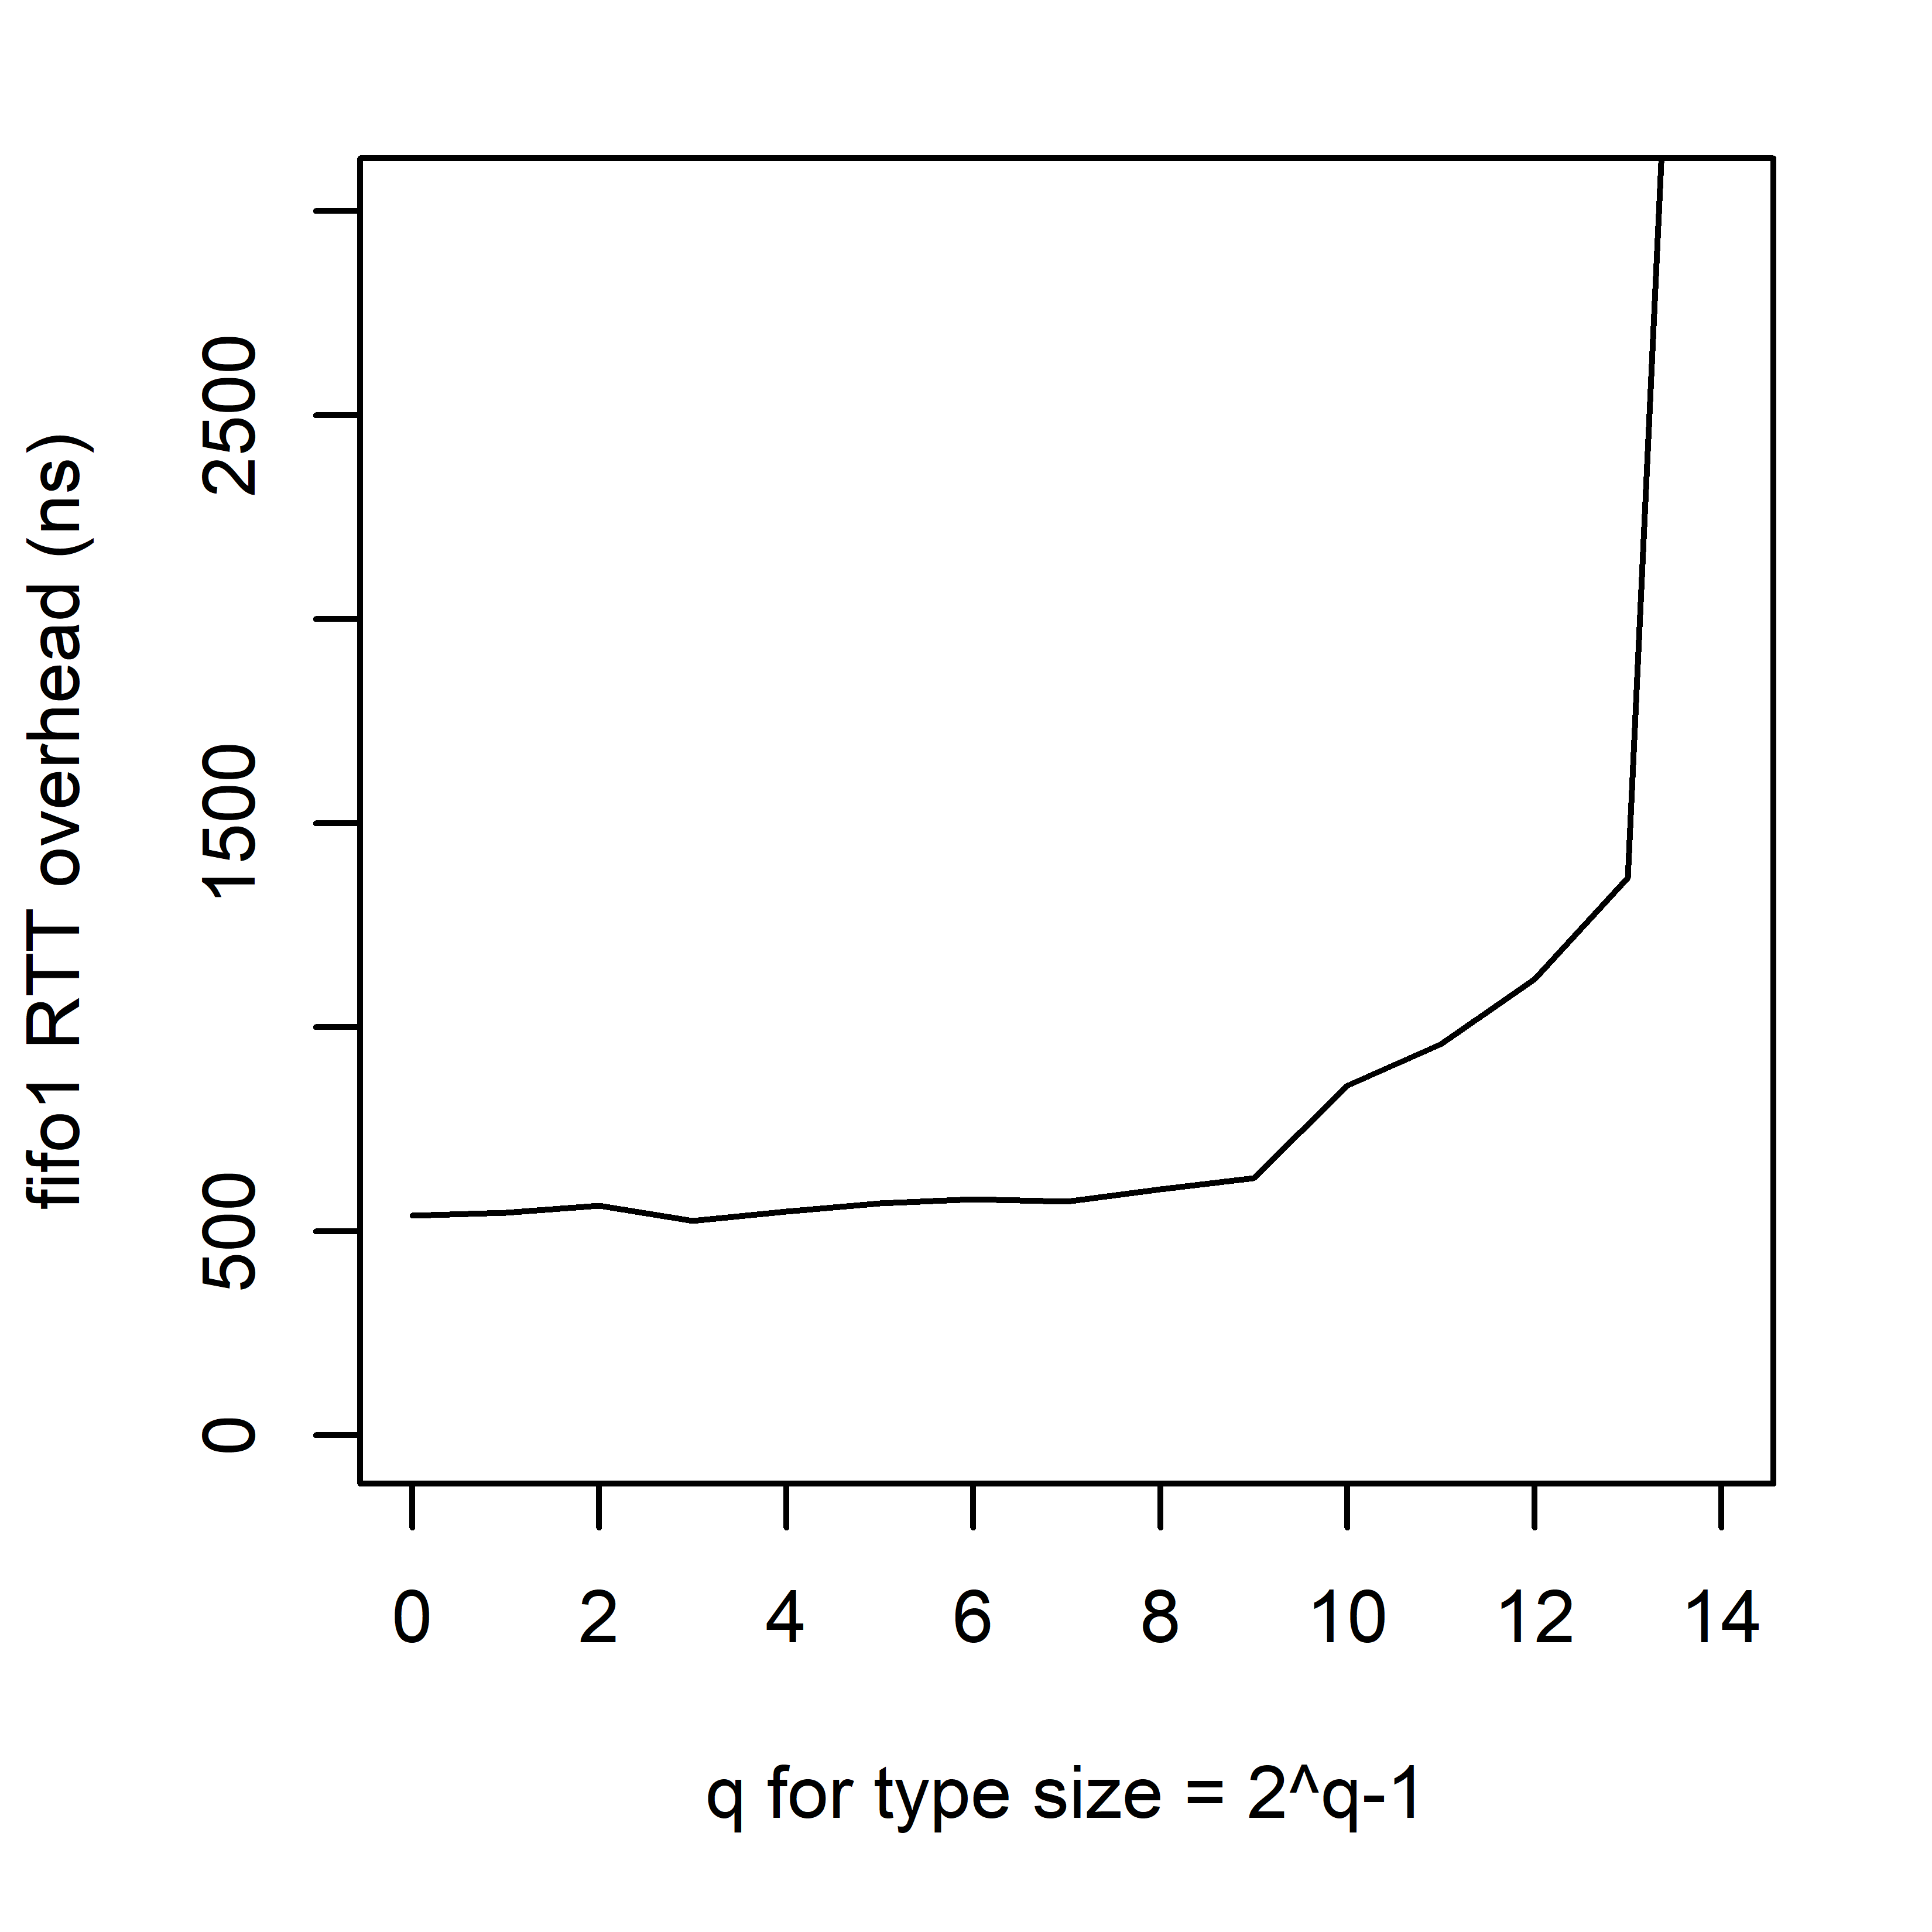
\includegraphics[width=\textwidth]{experiments/rtt_1.png}
			\caption{}
			\label{fig:exper_rtt_01}
		\end{subfigure}%
	}
	\caption[TODO]{TODO.}
	\label{fig:exper_rtt}
\end{figure}


\begin{figure}
	\centering
	\makebox[\textwidth][c]{
		\begin{subfigure}[b]{0.63\textwidth}
			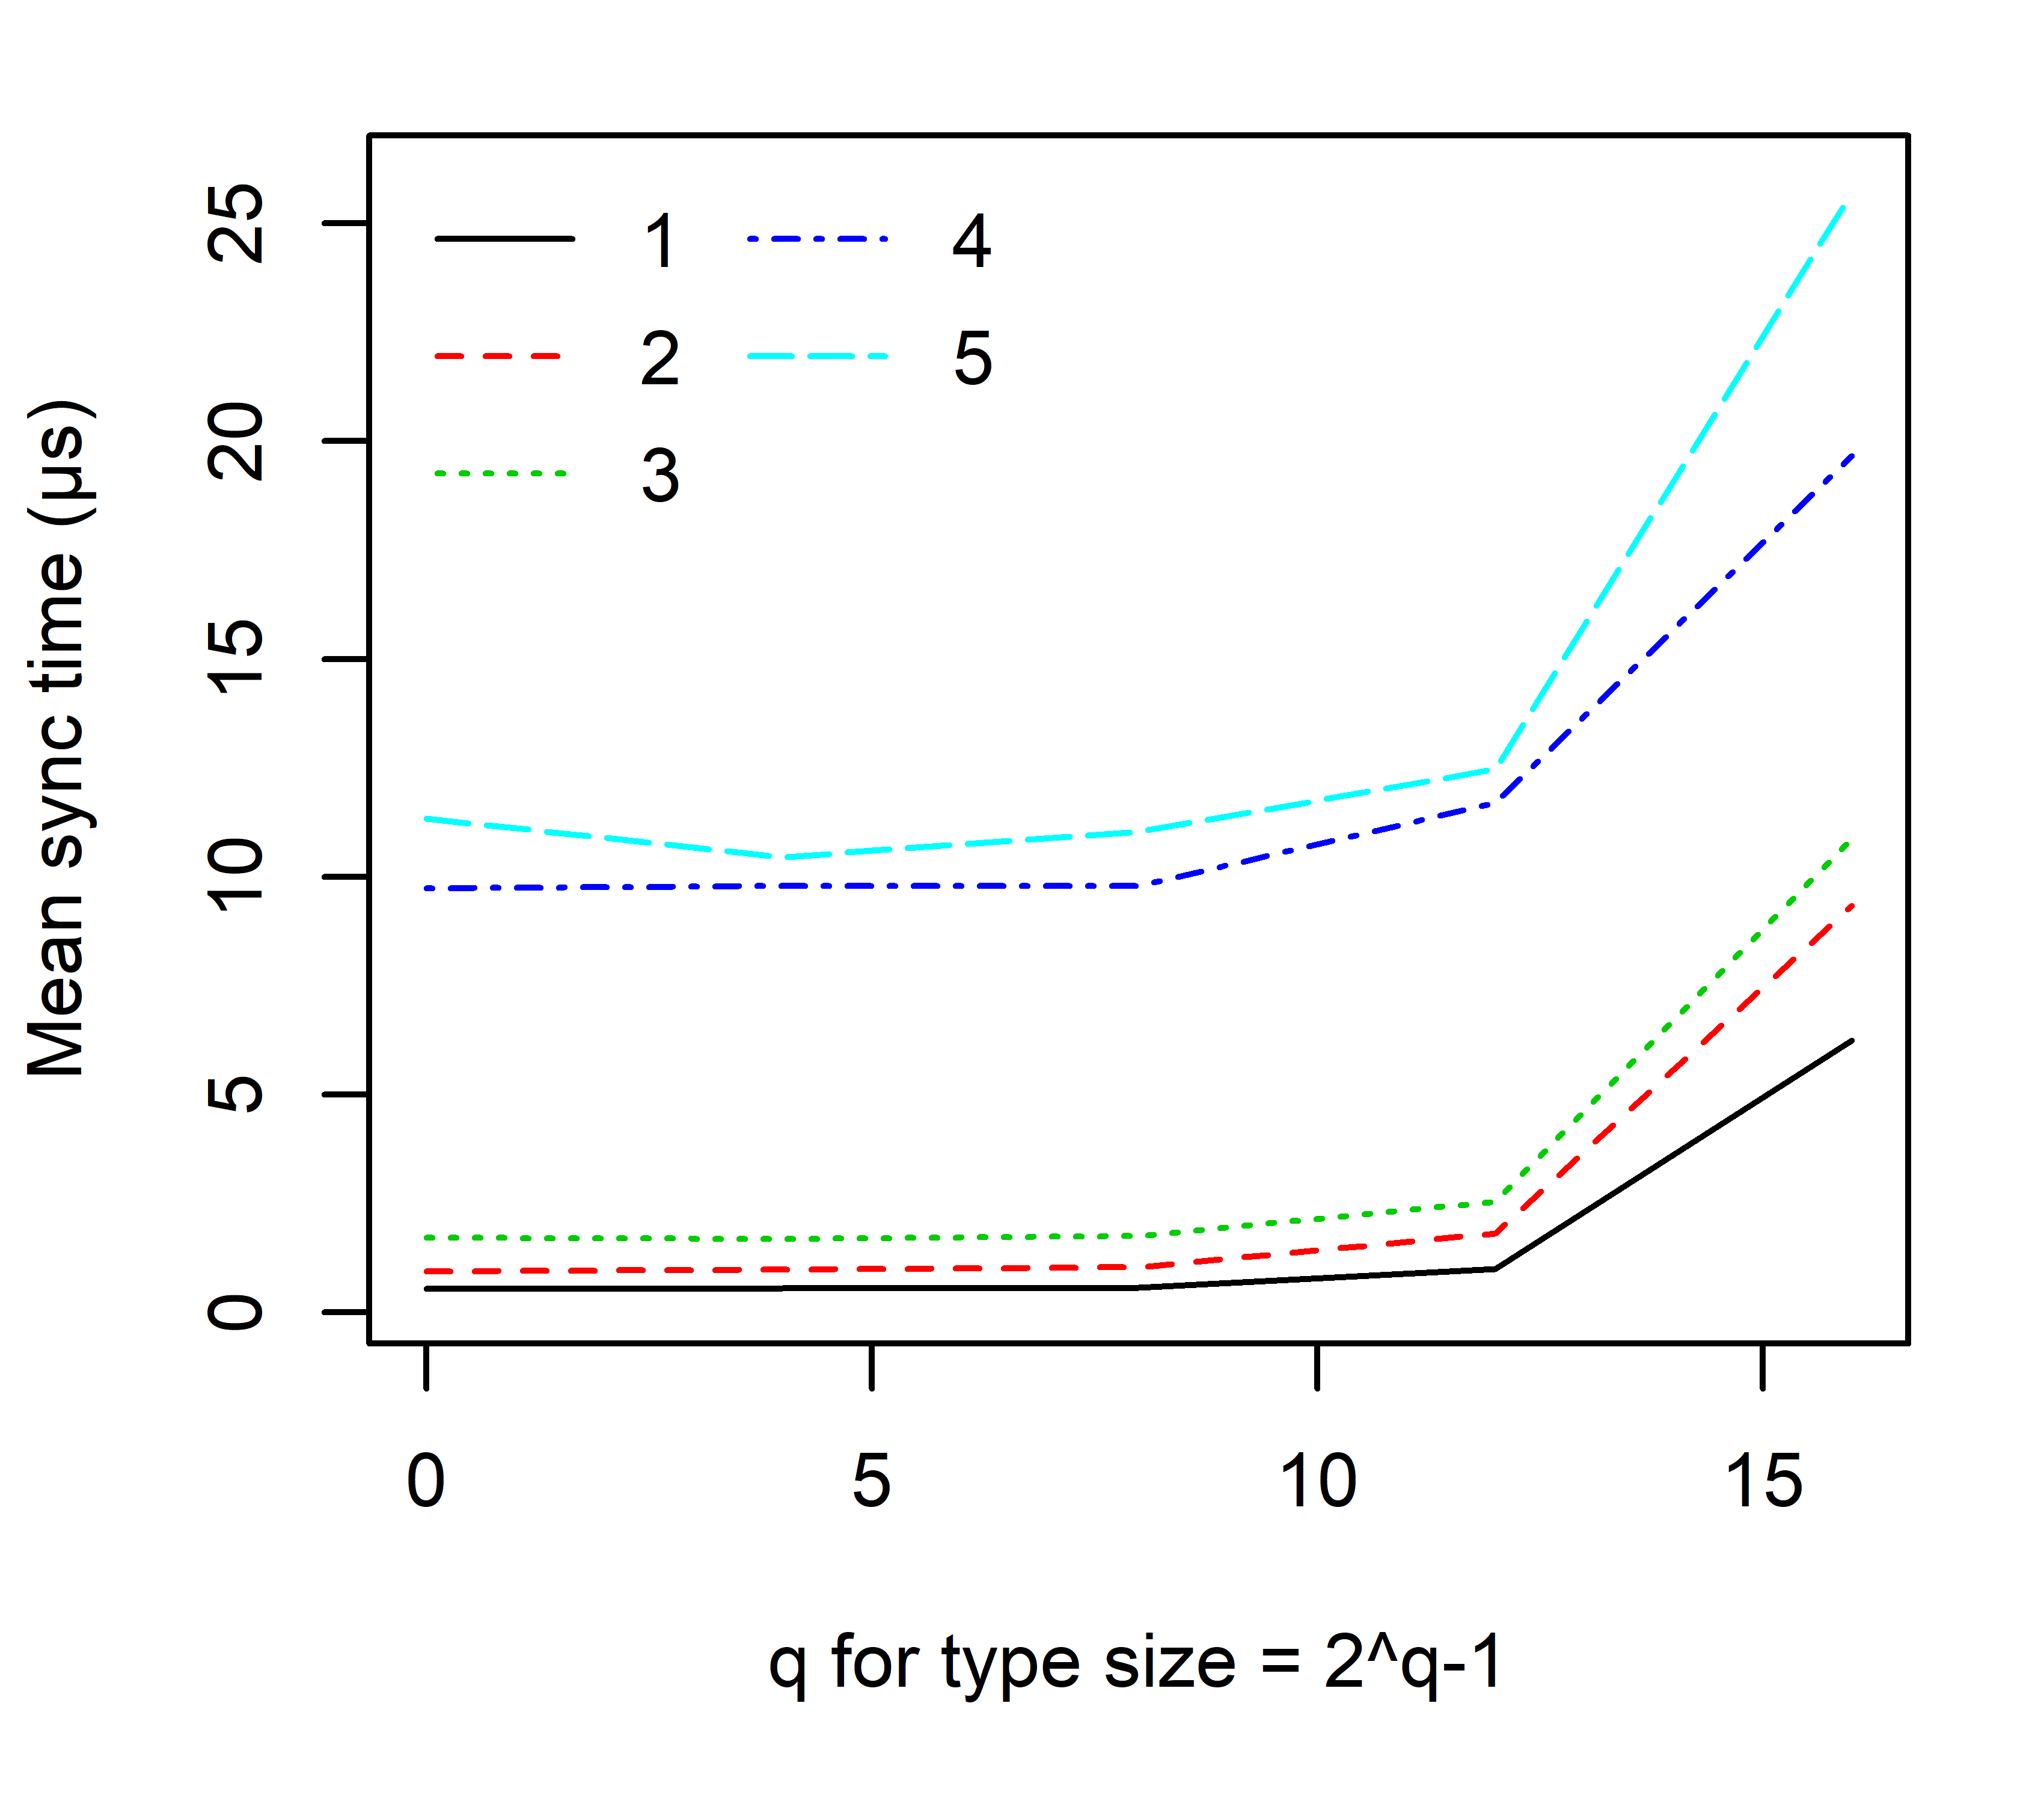
\includegraphics[width=\textwidth]{experiments/simo_copy_0.png}
			\caption{}
			\label{fig:simo_copy_0}
		\end{subfigure}%
		\begin{subfigure}[b]{0.63\textwidth}
			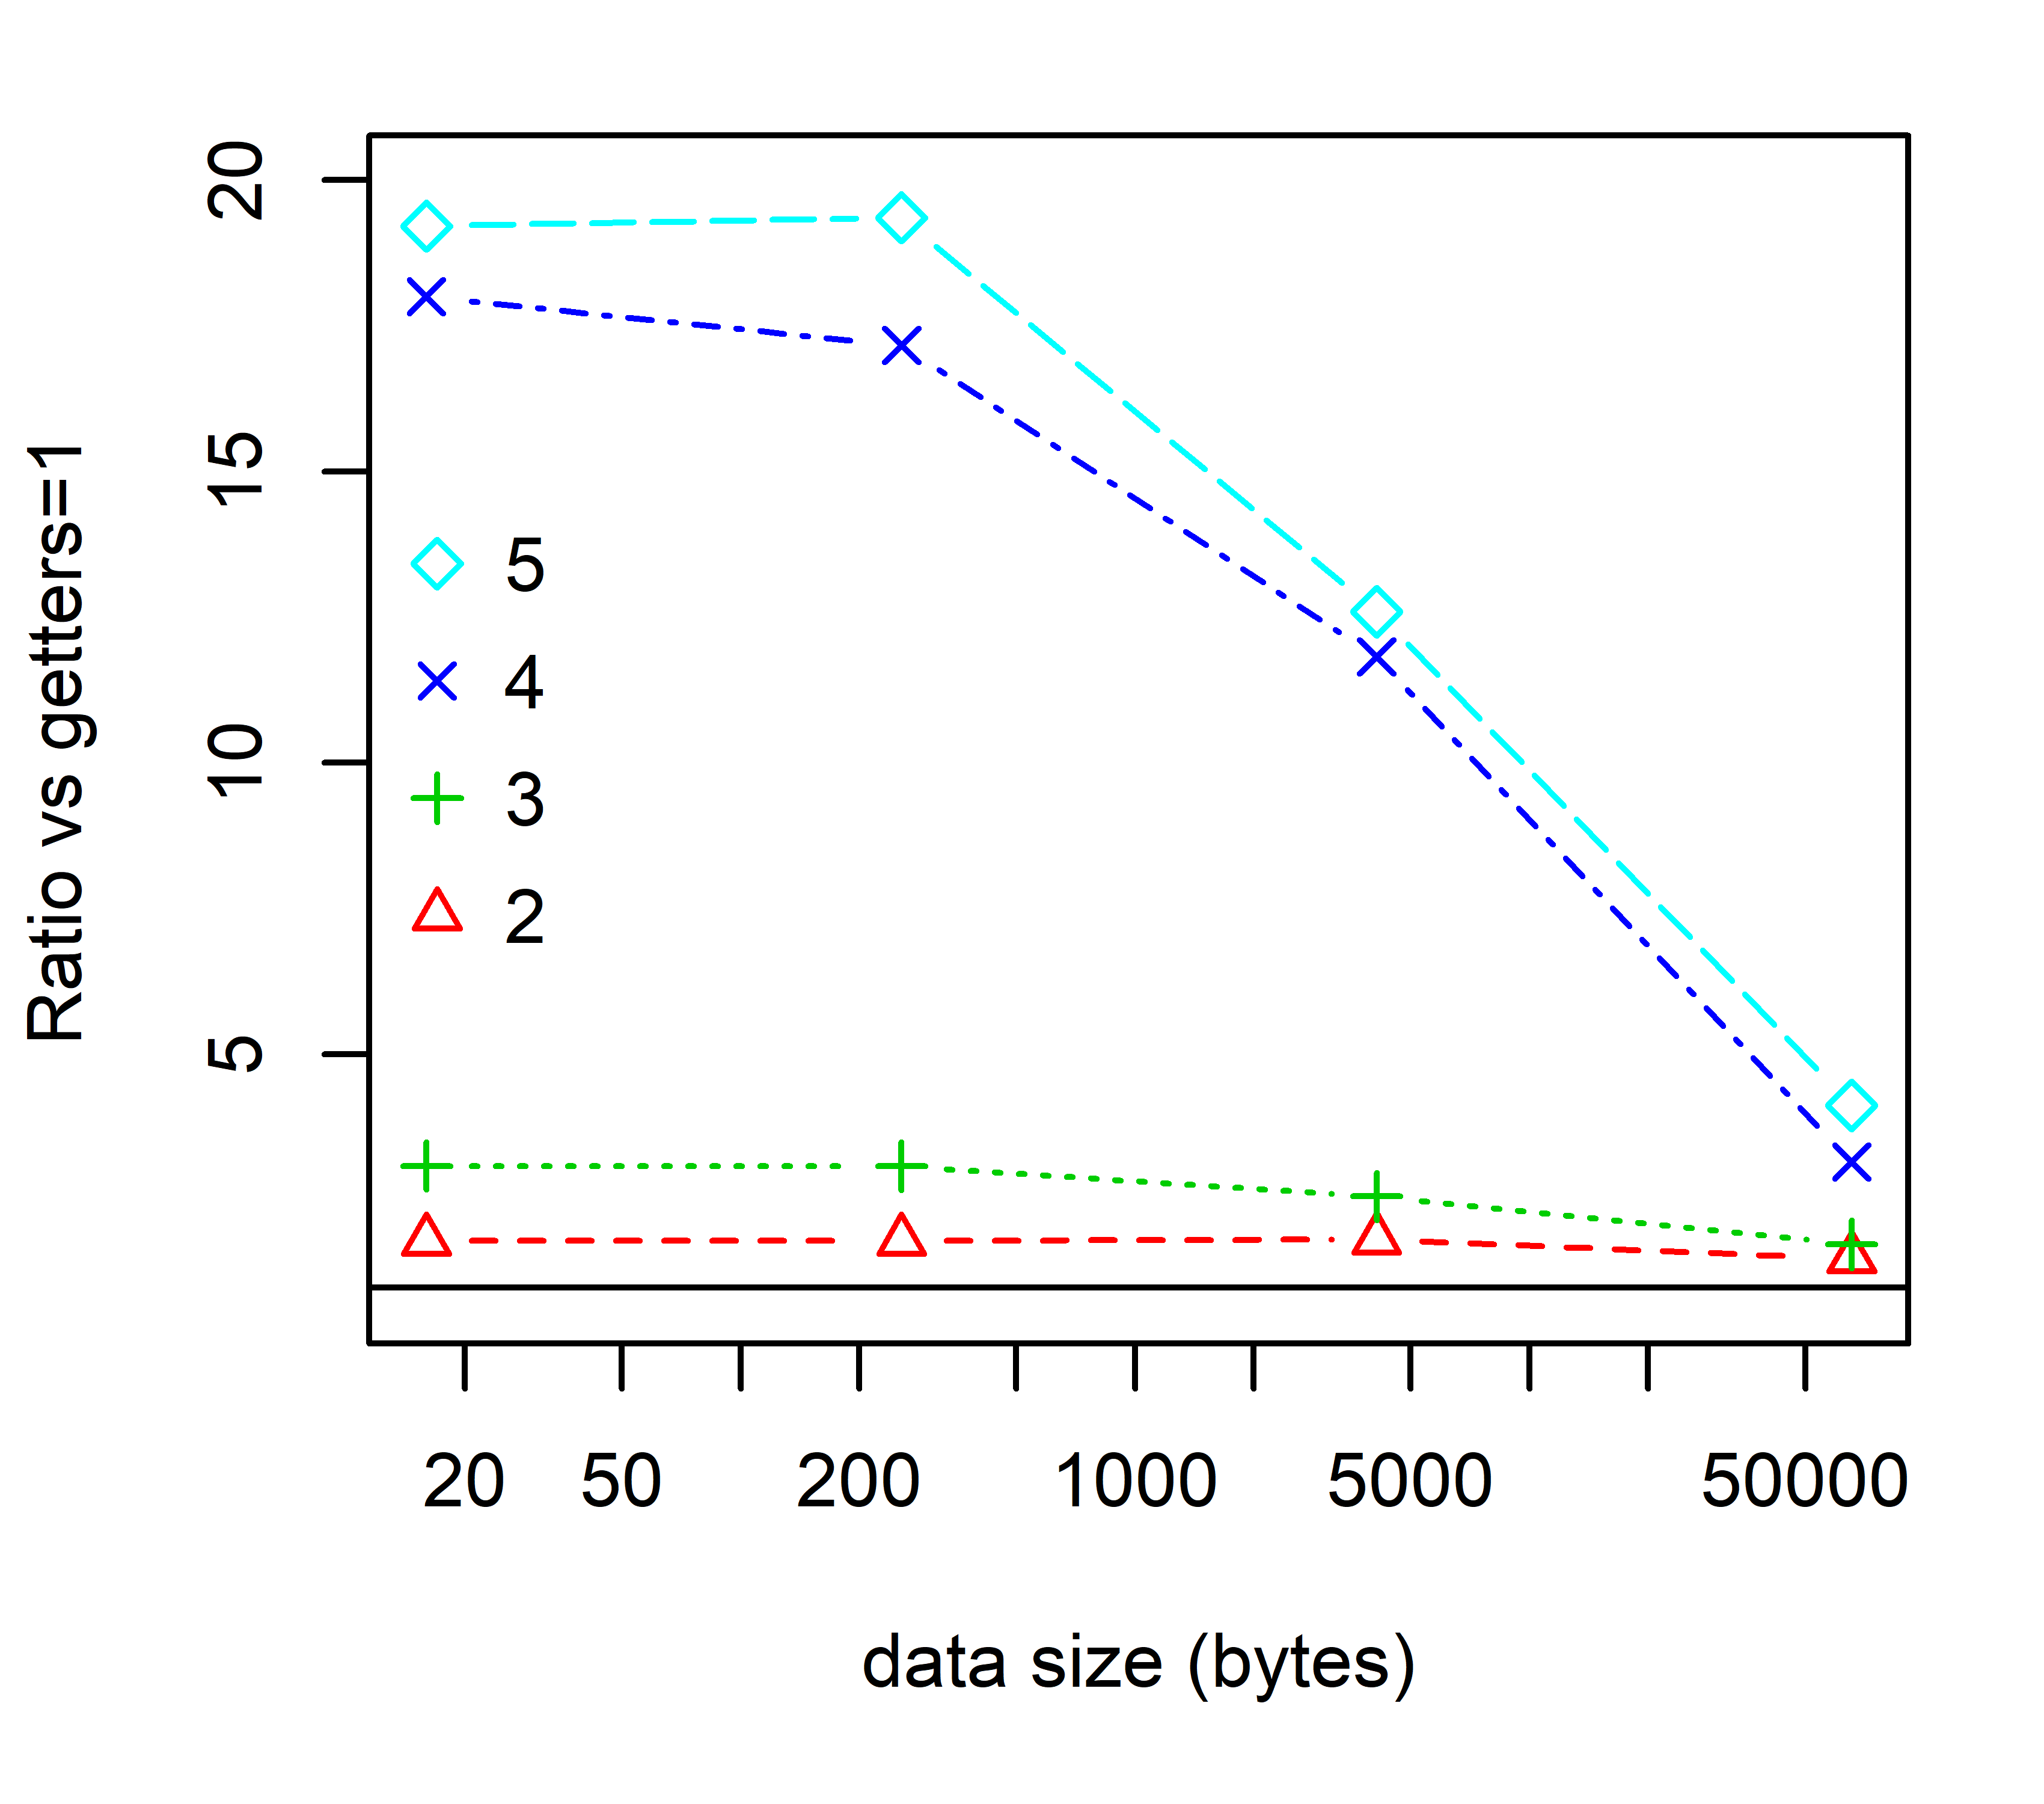
\includegraphics[width=\textwidth]{experiments/simo_copy_1.png}
			\caption{}
			\label{fig:simo_copy_1}
		\end{subfigure}%
	}
	\caption[TODO]{TODO.}
	\label{fig:simo_copy}
\end{figure}
\begin{figure}
\centering
\makebox[\textwidth][c]{
	\begin{subfigure}[b]{0.63\textwidth}
		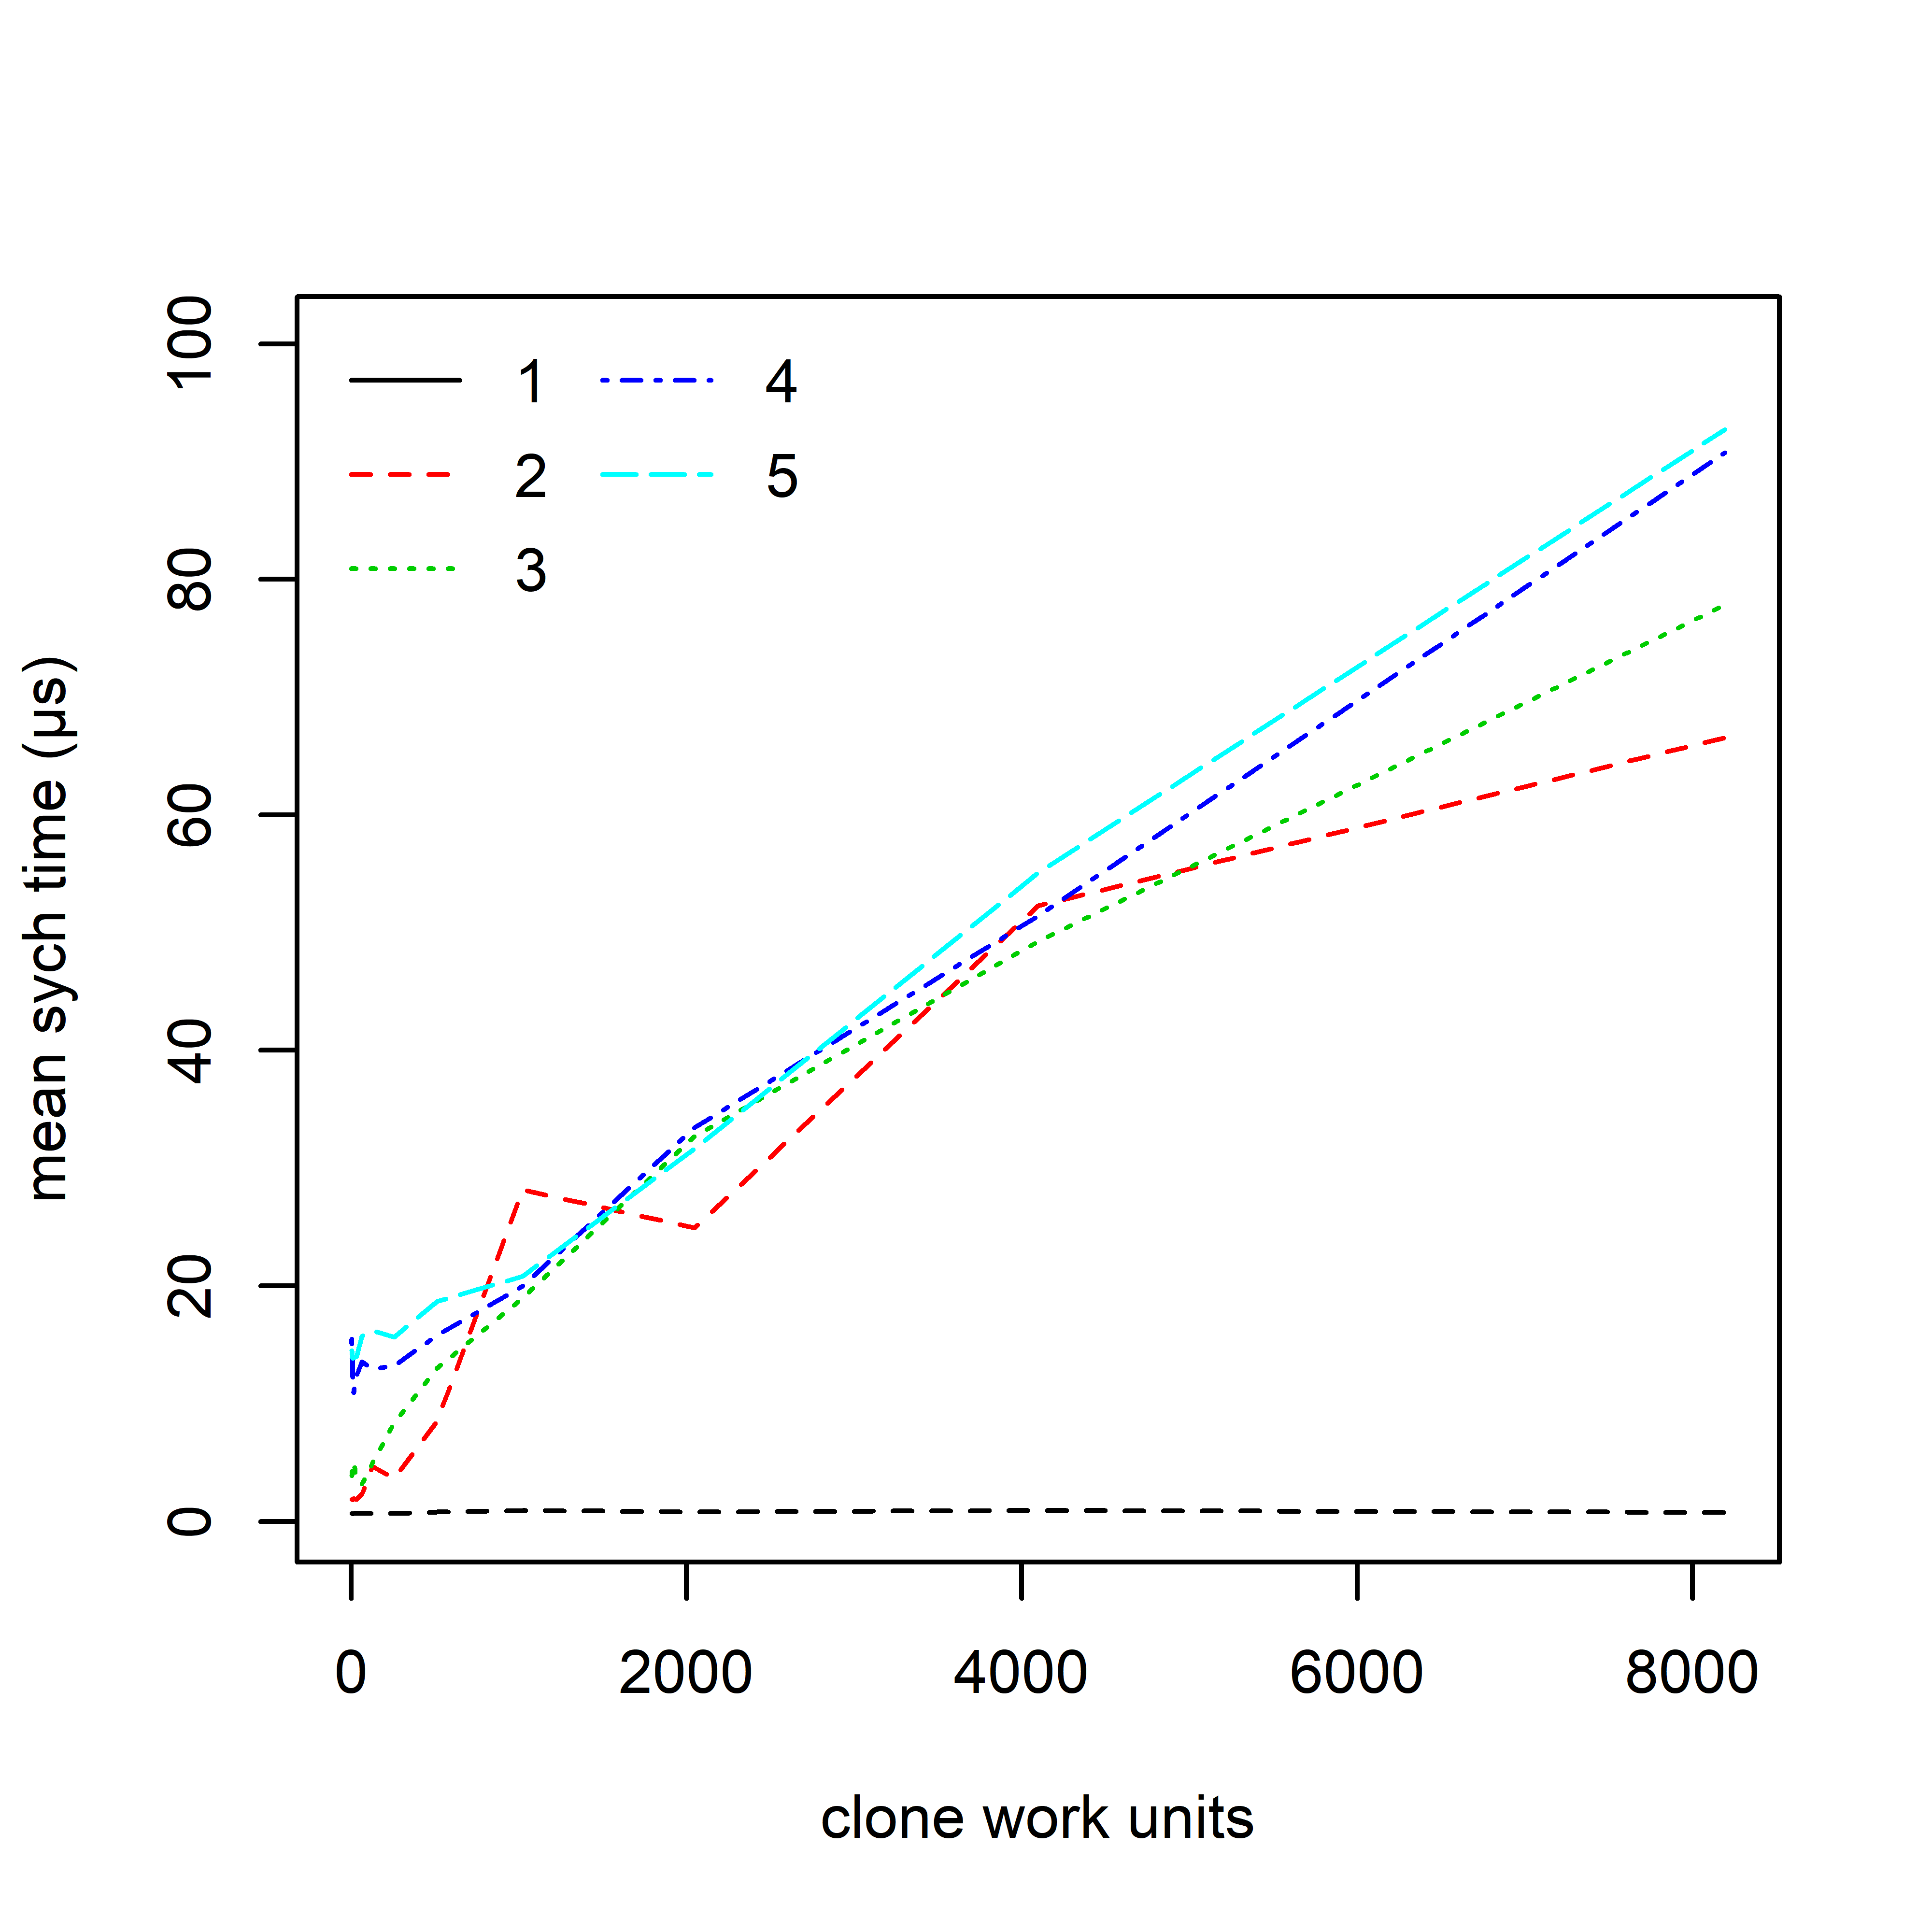
\includegraphics[width=\textwidth]{experiments/clone_compete_0.png}
		\caption{}
		\label{fig:clone_compete_0}
	\end{subfigure}%
	\begin{subfigure}[b]{0.63\textwidth}
		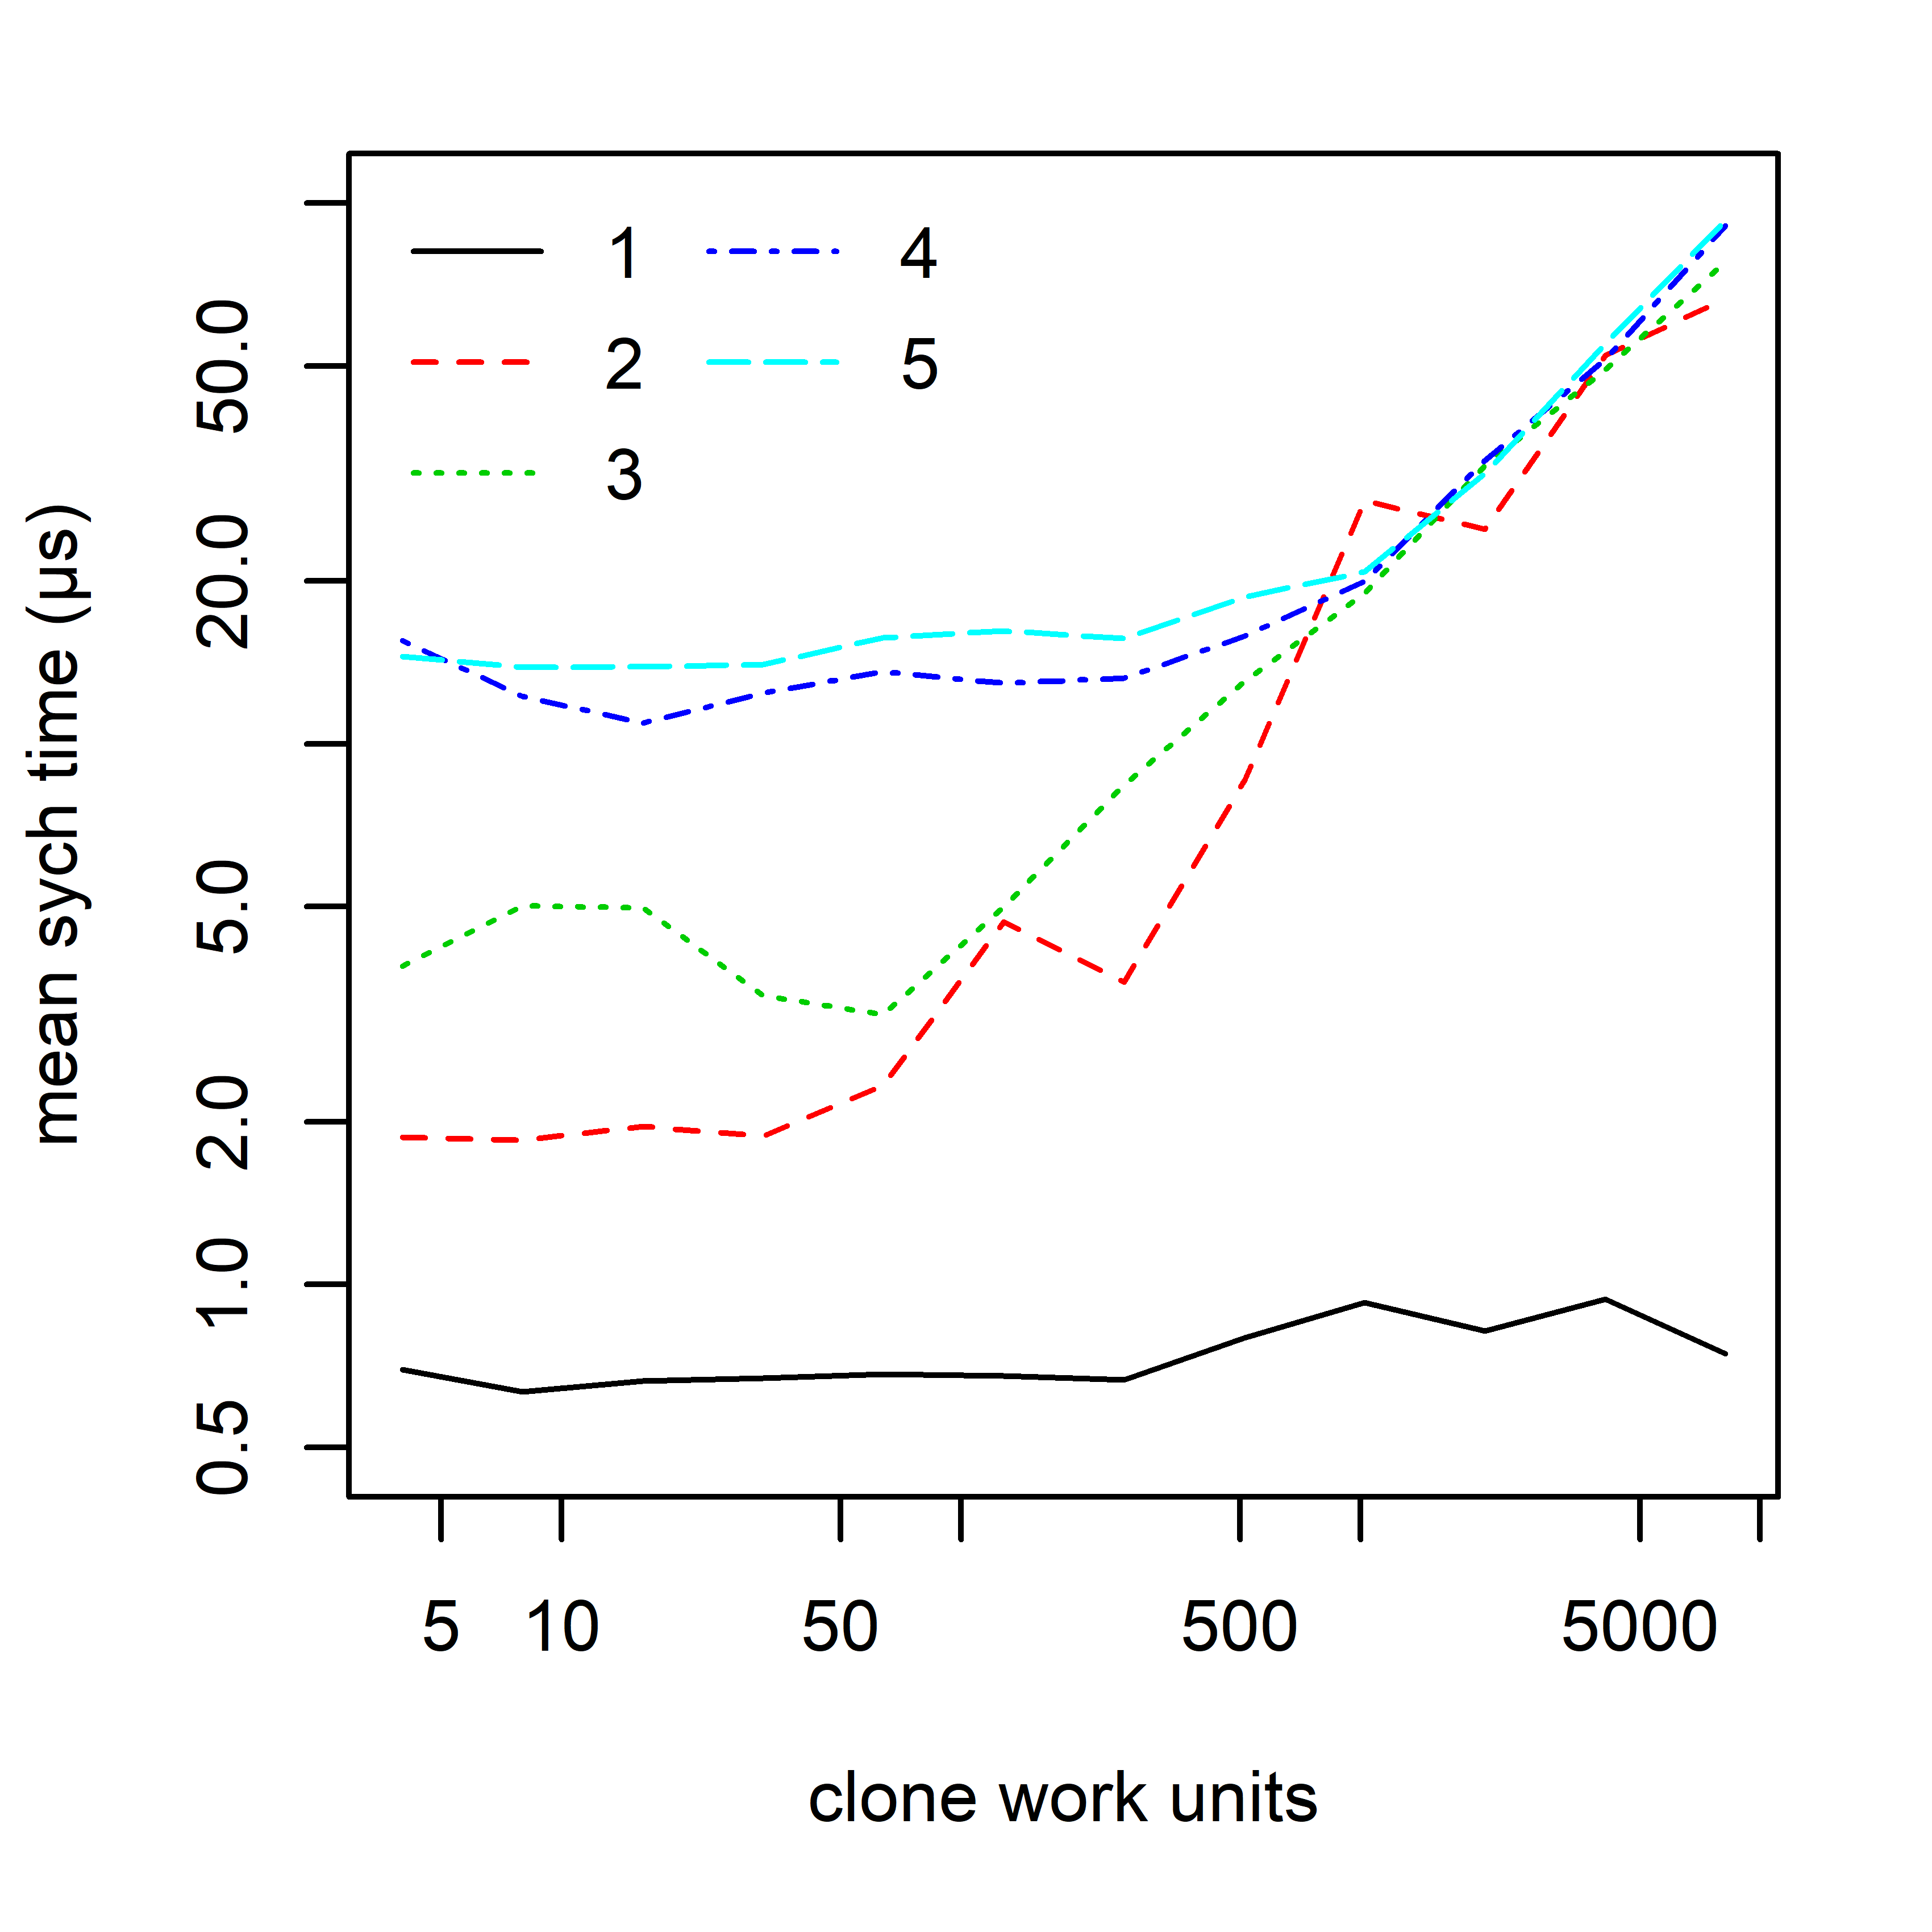
\includegraphics[width=\textwidth]{experiments/clone_compete_1.png}
		\caption{}
		\label{fig:clone_compete_1}
	\end{subfigure}%
}
\caption[TODO]{TODO.}
\label{fig:clone_compete}
\end{figure}
%

%
%\begin{figure}[t]
%	\centering
%	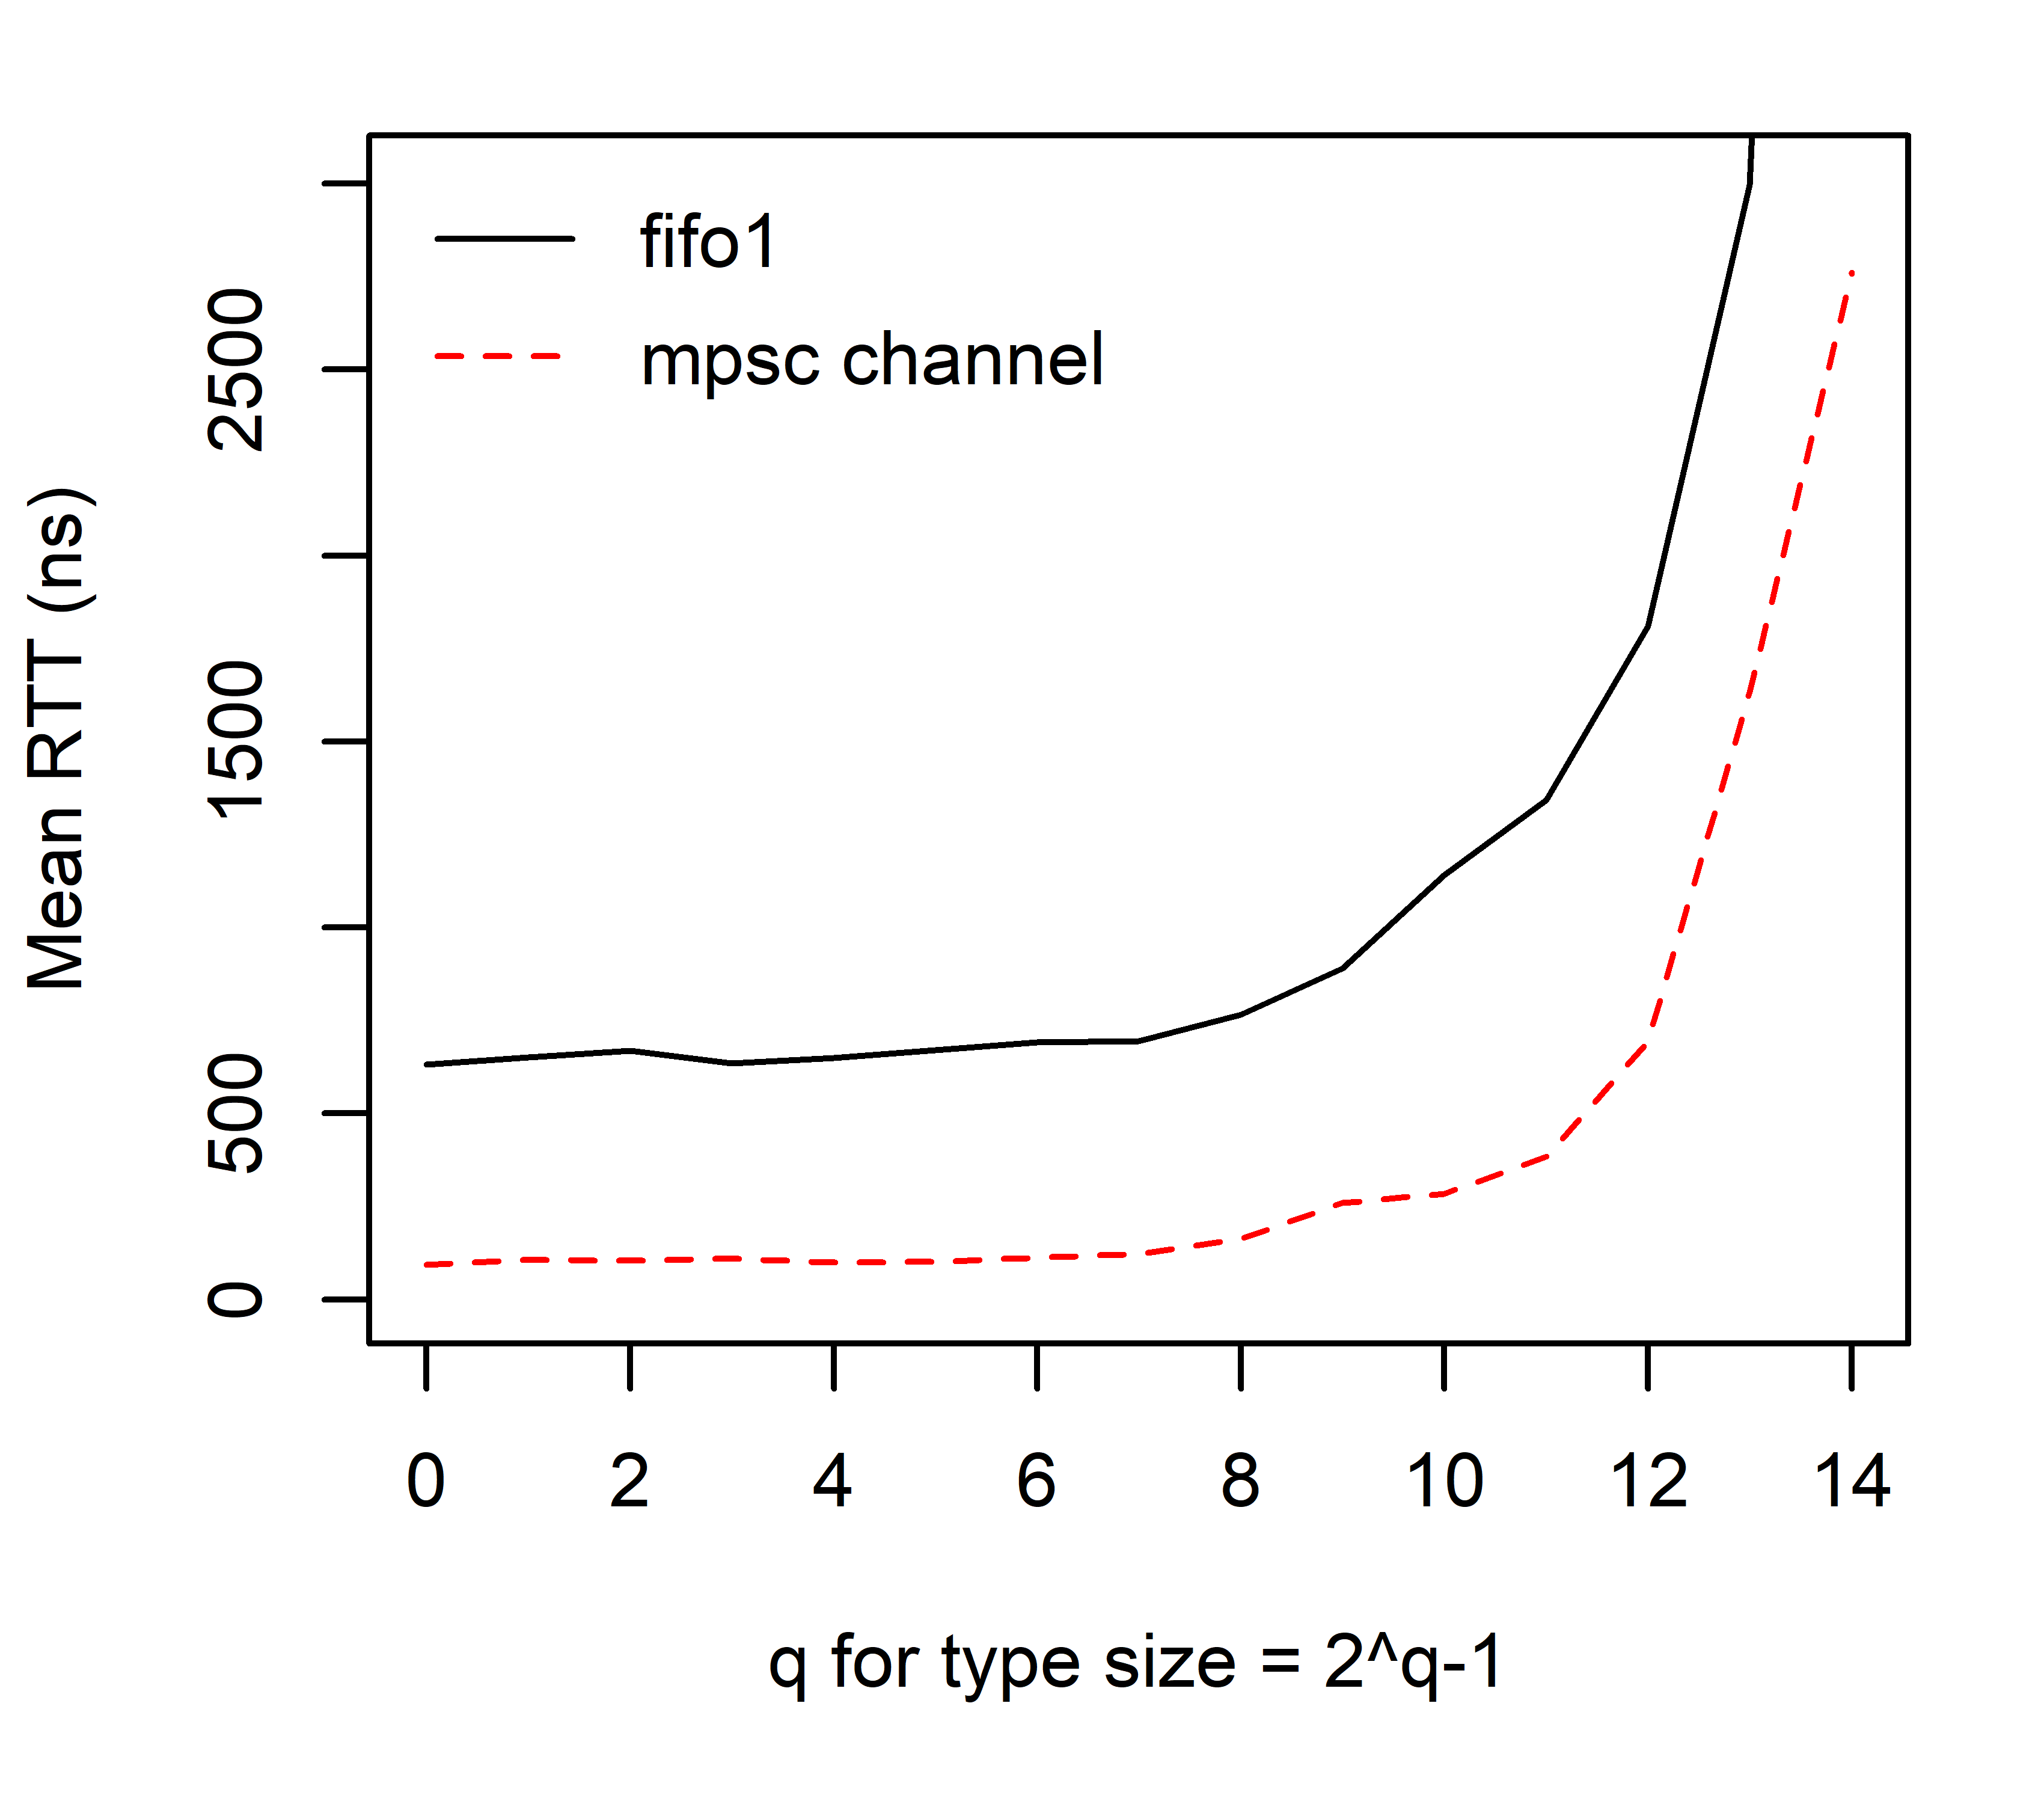
\includegraphics[width=8cm]{experiments/rtt_0.png}
%	\caption[TODO]{TODO}
%	\label{fig:exper_rtt_0}
%\end{figure}

\section{Observations}